\documentclass[12pt]{article}
\usepackage[left=0.5in, right=0.5in, top=0.75in, bottom=0.5in]{geometry}
\usepackage{epsfig,graphics,amsmath,color,multicol,enumitem,tabularx,pbox,url}
\usepackage{cancel}
%\usepackage[firstpage]{draft watermark}

\setlist{noitemsep}
\setlist{nolistsep}

\pagestyle{empty}

\begin{document}


\begin{tabular*}{\textwidth}{@{\extracolsep{\fill}}l l}
\textbf{Second Derivative}  &  Wizard name: \hrulefill \\
%\textbf{\today} & MATH 157, Hogwart's House: \rule{4cm}{0.5pt}  \\
\textbf{Math 160 } & MATH 160 Hogwart's House:\hspace{2cm} \\
\hline\hline
\end{tabular*} 

\small
{\em Learning Targets:
\begin{itemize}
\item Write the first, second and higher order derivatives using both prime and Leibniz notation.
\item Transfer connections between f and f ’ to f ’ and f ’’, and build connections between f and f ” (concavity).
\item Analyze information about the rate of change of f ' to draw conclusions about the concavity of f. 
\item Sketch the first and second derivative graphs given the graph of a function y = f(x).
\item Identify the intervals where a function is increasing and decreasing, concave up and concave down graphically. 
\item Compute the first and second derivatives of a power function using the power rule.
\item Interpret f ’ as velocity and f ” as acceleration. 
\end{itemize}

Aligns with Standards D3 and D4.}

\hrulefill

\normalsize 

\vspace{-.8cm}


\section*{Second Derivatives of Functions}

\begin{multicols}{2}
\begin{itemize}
\item Use a $\star$ to indicate a place on the graph where the function is increasing.
\item Use a $\diamond$ to indicate a place on the graph where $f'$ is negative.
\item What can you say about $f'(x)$ at the $\star$?
\item[]
\end{itemize}

 \vskip .5in
 
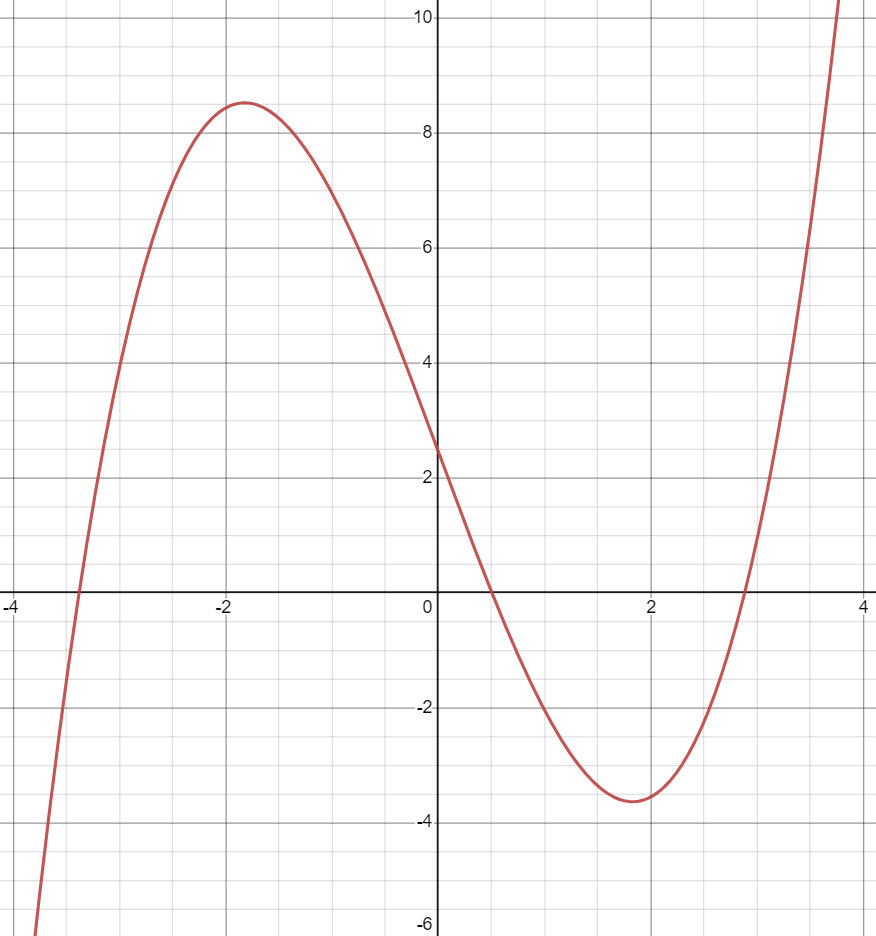
\includegraphics[scale=0.4, trim=0 80 0 50,clip]{cubic.png}
\end{multicols}

\hrulefill

\begin{multicols}{2}
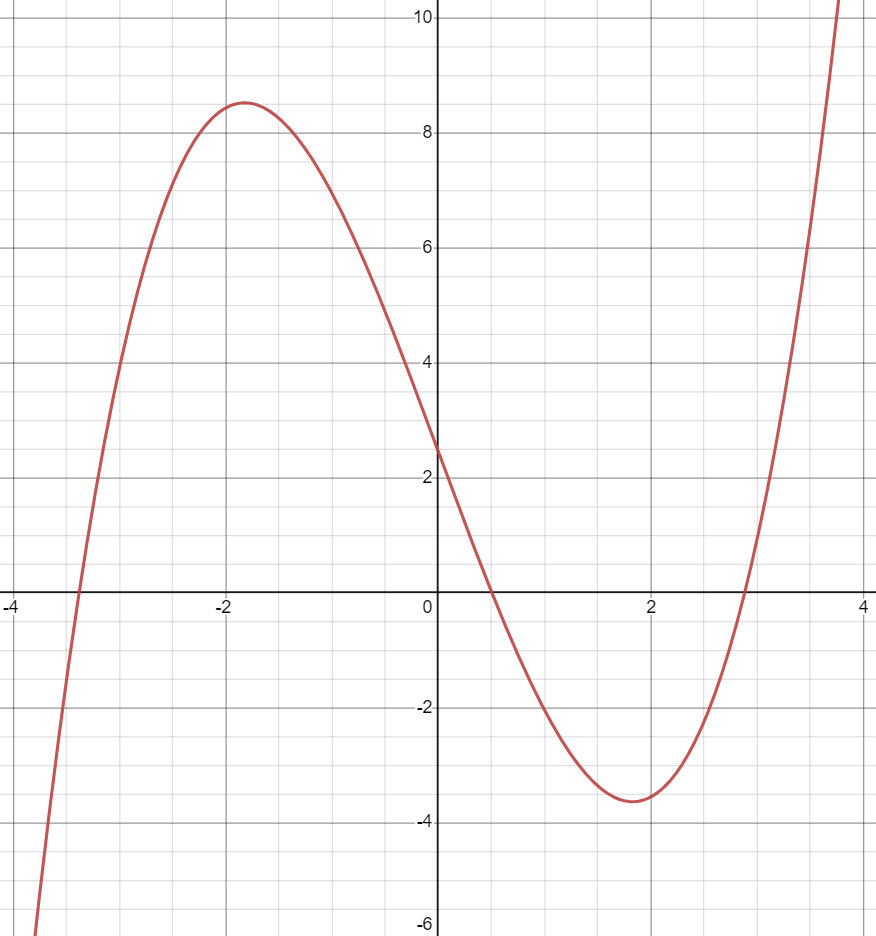
\includegraphics[scale=0.4, trim=0 80 0 50,clip]{cubic.png}

\begin{itemize}
\item Use a $\star$ to indicate a place on the graph where the derivative is positive and $x<0$.
\item Use a $\diamond$ to indicate a place on $f(x)$ where $f'$ is larger than $f'$ at the $\star$. It might help to think about steepness here.
\item Use a $\bigcirc$ to indicate a place on $f(x)$ where $f'$ is smaller than $f'$ at the $\star$. It might help to think about steepness here.
\item As $x$ increases, $f'(x)$ ... (Gets larger? gets smaller? Stays the same?)
%\item[]
\end{itemize}

% \vskip .5in
 
\end{multicols}

\hrulefill

\newpage

We can think about $f'(x)$ as a function, and we can think about computing the derivative of $f'$, and we could use that derivative to inform us about the behavior of $f'(x)$.

\begin{multicols}{2}
\begin{itemize}
\item Use a $\star$ to indicate a place on the graph where $f'$ is decreasing.
\item Use a $\diamond$ to indicate a place on the graph where $f'$ is increasing.
\item Use a $\bigcirc$ to indicate a place on the graph where $f'$ changes from decreasing to increasing?
\item[]
\end{itemize}

 \vskip .5in
 
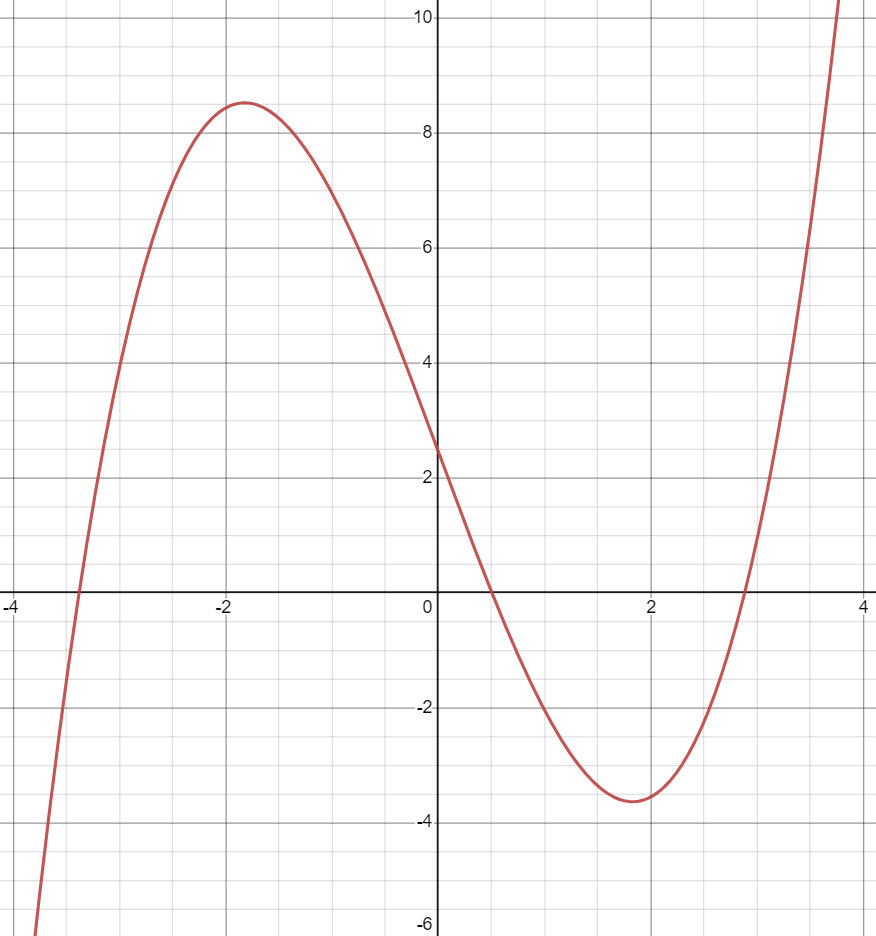
\includegraphics[scale=0.4]{cubic.png}
\end{multicols}

This can be a bit tricky because I'm asking you to think about the function and the derivative of $f'$ without much information in between the two.

Are there any words of phrases that help you think about where to place the dots?  

\hrulefill

\subsection*{Notation}

$f\left(x\right)$ represents the function. (The ``original'' function, or ``parent'' function can be helpful phrases sometimes.)

$f'\left(x\right)$ represents the first derivative. $f'(x)$ gives us information about how $f(x)$  is increasing or decreasing (or neither)

Other notation: $f'(x)$  can also be written $\displaystyle \frac{df}{dx}$

How can we talk about the derivative of the derivative?  Well, we could use Leibniz notation:

\vskip .1in

$\displaystyle \frac{d}{dx}f'\left(x\right)$ or $\displaystyle \frac{d}{dx}\ \frac{df}{dx}$ but we condense this notation as follows: $\displaystyle \frac{d^{2}f}{dx^{2}}$ and we call this the second derivative.

\vskip .1in

We can also use ``double prime'' notation: $f''\left(x\right)$

\begin{itemize}
\item $f(x)$ represents the function. (The "original" function, or "parent" function, gives output values on the graph.)
\item $f'(x)$ represents the first derivative. $f'(x)$ gives us information about how $f(x)$ is increasing or decreasing (or neither)
\item $f''(x)$ represents the second derivative. $f''(x)$  gives us information about how $f'(x)$ is increasing of decreasing. \newpage

\item If $f'(x)>0$, $f(x)$ is \rule{8cm}{0.5pt} \vskip .2in
\item   If $f'(x)<0$, $f(x)$ is \rule{8cm}{0.5pt} \vskip .2in 
\item If $f''(x)>0$, $f'(x)$ is \rule{8cm}{0.5pt} \vskip .2in
\item  If $f''(x)<0$, $f'(x)$ is \rule{8cm}{0.5pt} \vskip .2in
\end{itemize}



But what does $f''(x)$ tell us about $f(x)$?

\begin{multicols}{2}
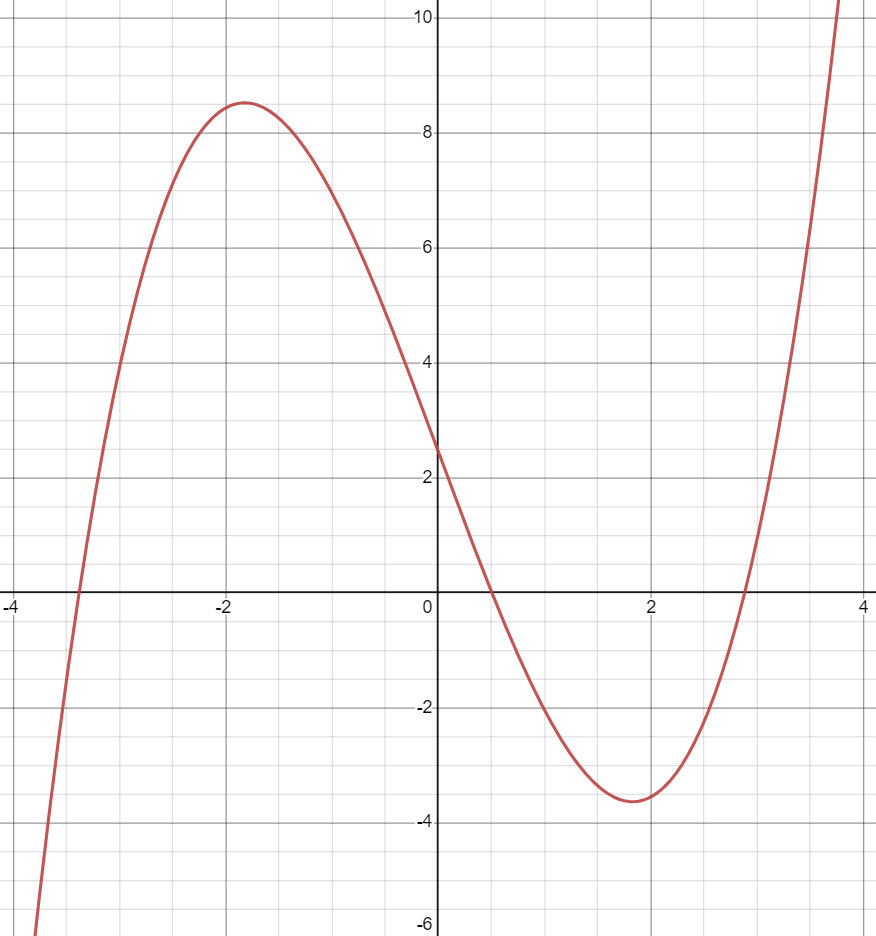
\includegraphics[scale=0.4]{cubic.png}

\begin{itemize}
\item Sketch several tangent lines on this graph.
\item Notice where the tangent lines are below the curve.
\item Notice where the tangent lines are above the curve.
\item Use a $\bigcirc$ to indicate a place on the graph where the tangent lines change from begin above or below.
\item Do the $\bigcirc$ symbols that you drew show up in the same locations as the previous graph?
\end{itemize}


 
\end{multicols}
 \vskip .5in
 
 \subsection*{Concavity}
 
 Concavity is the word we use to describe how the function is curving. 
 
If the function is opening upward, we describe the function as concave up.
 
If the function is opening downward, we describe the function as concave down.

\vskip .5in
\begin{itemize}[parsep=2in]
\item Sketch the graph of a function that is always concave up. \newpage
\item Sketch the graph of a function that is always concave down.
\item Sketch the graph of a function that is always increasing and concave down.
\item Sketch the graph of a function that is always increasing and concave up.
\item Sketch a graph that represents the following idea:
When I'm running at first I have a lot of energy so I run really fast, but as I get tired I start to slow down.
Sketch a graph that represents the distance this person has run. (assume they are running in a straight line.
What does the concavity of this graph tell you?  Does it make sense to align concavity with acceleration? \newpage
\item Can an object have negative velocity but positive acceleration?
Either sketch an example or describe the example with words.
\end{itemize}

\vskip 2.5in

It is very important to be fluent with all the different ways we can understand the behavior of a graph based off of information about $f$, $f'$ and $f''$.



I strongly suggest you make a chart or table summarizing how $f$, $f'$ and $f''$ are related to each other.  Look at what a positive derivative tells you about $f$. What does a positive second derivative tell you about $f'$? about $f$?  Behavior we typically care about: increase/decrease and concavity. 


Everything that $f'$ can tell you about $f$, $f''$ can also tell you about $f'$.

\vskip .2in

Recall the power rule: $\frac{d}{dx}ax^b = abx^{b-1}$ where $a$ and $b$ are constants and $x$ is the variable.

We can compute the second derivatives by taking the derivative twice:

$$\frac{d^2}{dx^x} f(x)=\frac{d}{dx} \frac{d}{dx} f(x) = f''(x)$$

\begin{enumerate}
\item Compute the following derivatives:

\begin{enumerate}
\item $\displaystyle \frac{d^2}{dx^2} 4x^5=$ \vskip 1in
\item  $\displaystyle \frac{d^2}{dx^2} \frac{1}{\sqrt{x}}$= 
\end{enumerate}

\newpage

%%CURVE SKETCH%%

\item Sketch the graph of a function defined on $[0,8]$ that has all of the following properties:

\begin{itemize}
\begin{multicols}{2}
\item $\displaystyle f'(x)>0$ for $0<x<4$
\item $\displaystyle f'(x)<0$ for $x>4$
\item $\displaystyle f''(x)<0$ for $4<x<6$
\item $\displaystyle f''(x)>0$ for $x>6$
\item $f(x)$ is continuous on $0\leq x\leq 8$
%\item $f'(x)$ is undefined at $x=4$
\item $f(4)=6$
\item $f(6)=2$
\end{multicols}
\end{itemize}

\vspace{2cm}

%\begin{center}
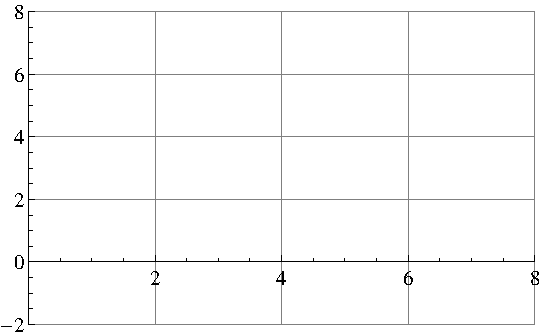
\includegraphics[scale=1.5]{grid.pdf}
%\end{center}

%\underline{\hspace{7in}}



\newpage

 A function $f(x)$ and its first and second derivatives are graphed below.  We need to identify which curve belongs to which function.
 
 \begin{multicols}{2}
 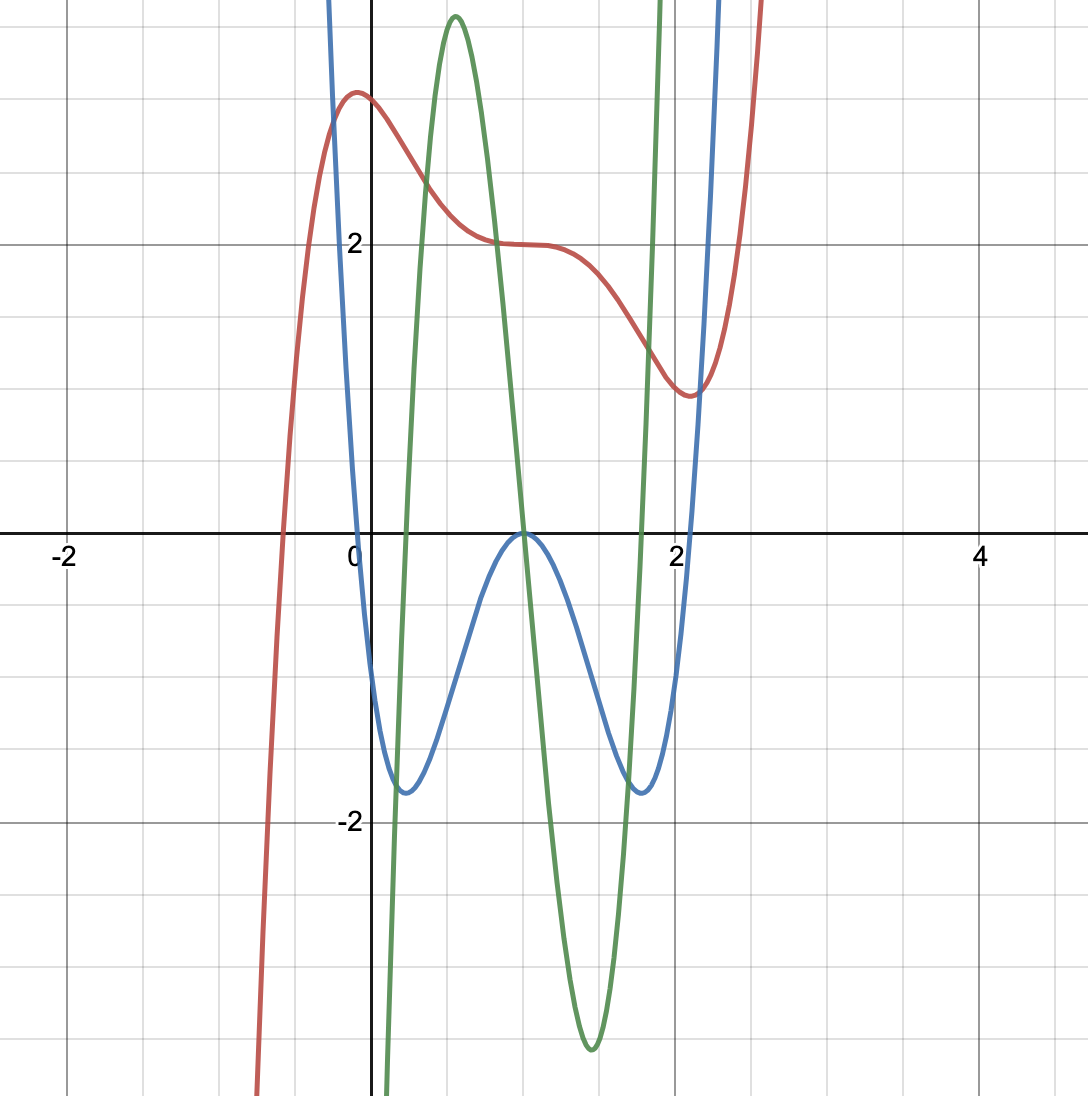
\includegraphics[scale=.5]{curvematch1.png}
 
 \begin{itemize}[parsep=.1in]
 \item Label the graphs $A$, $B$ and $C$.
 \item Identify where each graph has a horizontal tangent line (in other words, where the derivative of that graph would be zero.) Do any other graphs cross the $x$-axis at the same $x$-values where the slope would be zero?
 \item Identify where each graph is increasing and where it is decreasing.
\item  Identify where each graph has positive outputs and negative outputs.
\item Identify where each graph is concave up and concave down. 
 \end{itemize}
 
 \end{multicols}

Write sentences like:\\

\begin{itemize}[parsep=.2in]
\item Graph A is increasing when $x$ is between
\item Graph A is decreasing when $x$ is between
\item Graph A has zero slope when $x$ is
\item Because Graph \rule{1cm}{0.5pt} is positive when Graph A is increasing AND negative when Graph A is decreasing AND is zero when Graph A has zero slope,  I know that Graph A's derivative is Graph \rule{1cm}{0.5pt} .
\end{itemize}

\vskip .1in
Repeat the reasoning for two other graphs.
\vskip .1in
Then write sentences like:\\
\begin{itemize}[parsep=.2in]
\item Graph A is concave up when $x$ is between
\item Graph A is concave down when $x$ is between
\item Graph A changes concavity when $x$ is
\item Because Graph \rule{1cm}{0.5pt} is positive when Graph A is concave up AND negative when Graph A is concave down AND is zero when Graph A is changing concavity,  I know that Graph A's {\em second} derivative is Graph \rule{1cm}{0.5pt} .
\end{itemize}

\vskip .1in
Repeat the reasoning for two other graphs.



\end{enumerate}

\end{document}
